\newpage

\section{Using the CPX/CPB as a Data Acquisition System (DAQ)}
\label{s:daq}

\subsection{Parts List}

\begin{enumerate}[itemsep=-5pt]
\item Laptop
\item CPX/CPB
\item USB Cable
\end{enumerate}

\subsection{Learning Objectives}
\begin{enumerate}[itemsep=-5pt]
\item Record real time measurements from the CircuitPlayground using the Serial monitor
\item Learn how to use the typing module to type data directly into a spreadsheet or text file
\item Learn how to log data on the on board memory of the CircuitPlayground 
\end{enumerate}

\subsection{Extra Help}

This is a pretty hard project to do with multiple different
methods. After you’ve read through this document I suggest you watch
a youtube I created on \href{https://youtu.be/yX0zeIfn2j4}{Logging Data with the Circuit Playground
Express}. I have also made video where I \href{https://www.youtube.com/watch?v=Vc7_KxRnORI}{log temperature and
accelerometer data using on board memory with the CircuitPlayground
Bluefruit.}

\subsection{Getting Started}

Taking data is the core of any instrumentation project. Data
Acquisition Systems or DAQ for short come in all shapes and
sizes. Believe it or not the CPX can be used as a crude and cheap
DAQ. The CPX can easily take temperature data and monitor the
temperature in a greenhouse or take humidity readings of a plant to
monitor soil content. Before we learn about the different sensors on
board the CPX, we want to make sure we can store that data later
rather than just having it spit data out via the serial monitor. For
starters though let’s get the CPX to print out something simple like
button presses since we’ve touched on that already. The code I’m using
is shown below and can also be found on
\href{https://github.com/cmontalvo251/Microcontrollers/blob/master/Circuit_Playground/CircuitPython/Data_Logging/button_presses.py}{Github}.
\begin{figure}[H]
  \begin{center}
    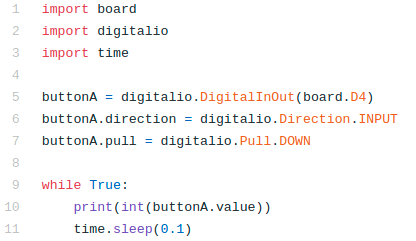
\includegraphics[width=\textwidth]{Figures/button_presses.png}
  \end{center}
\end{figure}
The code is pretty similar to what I had in the past. I import board,
digitalio, and time. I create a buttonA object using the digitalio
library to record button presses. I then enter into a while loop print
the buttonA.value. The difference here is that I use the int()
function to convert the buttonA.value to an integer. The reason why I
do this is because buttonA.value is a boolean. It is either True or
False. An integer though is a number and thus a value of False is 0
and True is 1. If you open the serial monitor and push the A button
down a few times you’ll see some zeros and 1’s.
\begin{figure}[H]
  \begin{center}
    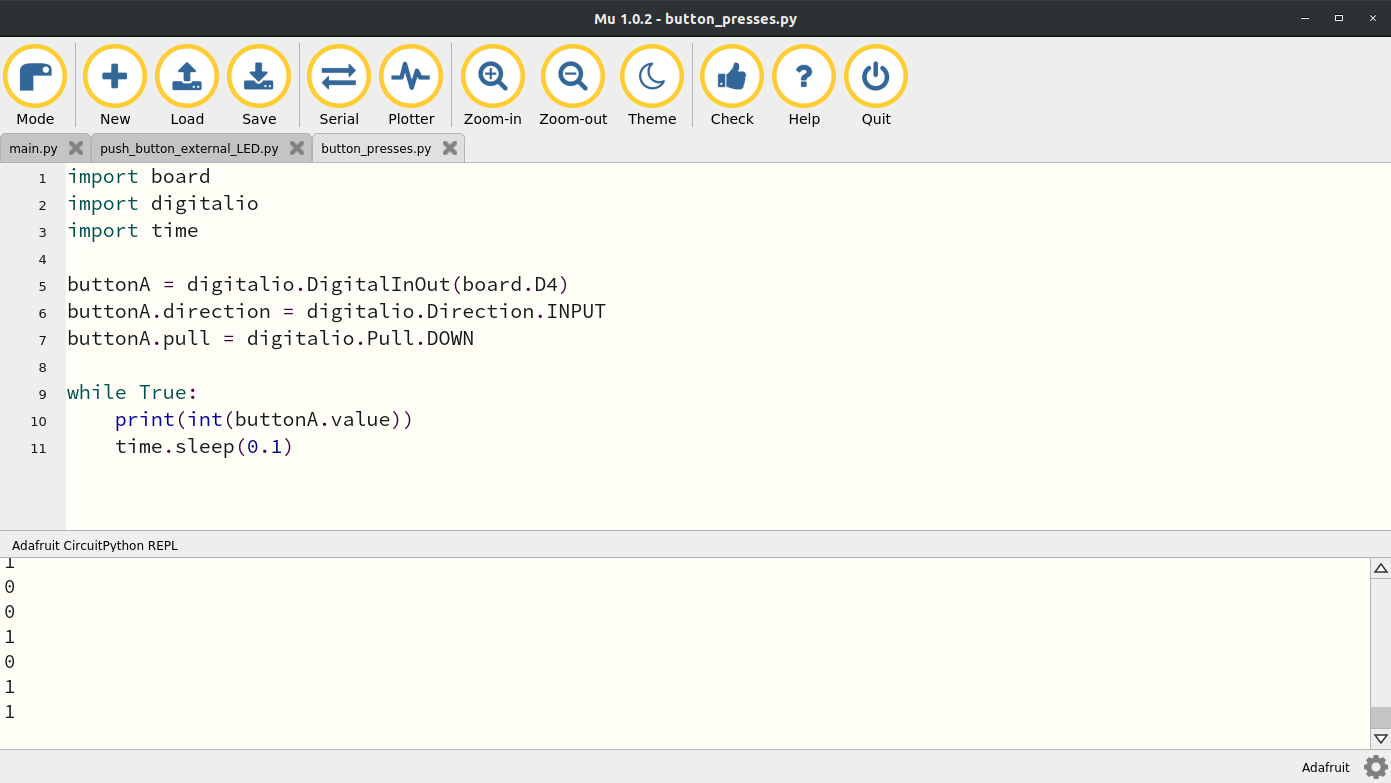
\includegraphics[width=\textwidth]{Figures/MuButtonPress.png}
  \end{center}
\end{figure}
Mu also has a really neat builtin plotter. You’ll see next to the
Serial button there is a button called Plotter. If you click that
button now nothing will pop up on the screen. Unfortunately in order
to plot using the Plotter you need to modify the print() statement to
this:
\begin{verbatim}
print((int(buttonA.value),))
\end{verbatim}
Notice the extra parentheses and the comma. Now if you click Plotter
you’ll see something like this. You’ll notice that the print statement
now has commas in it and the Plotter is recording button presses. 
\begin{figure}[H]
  \begin{center}
    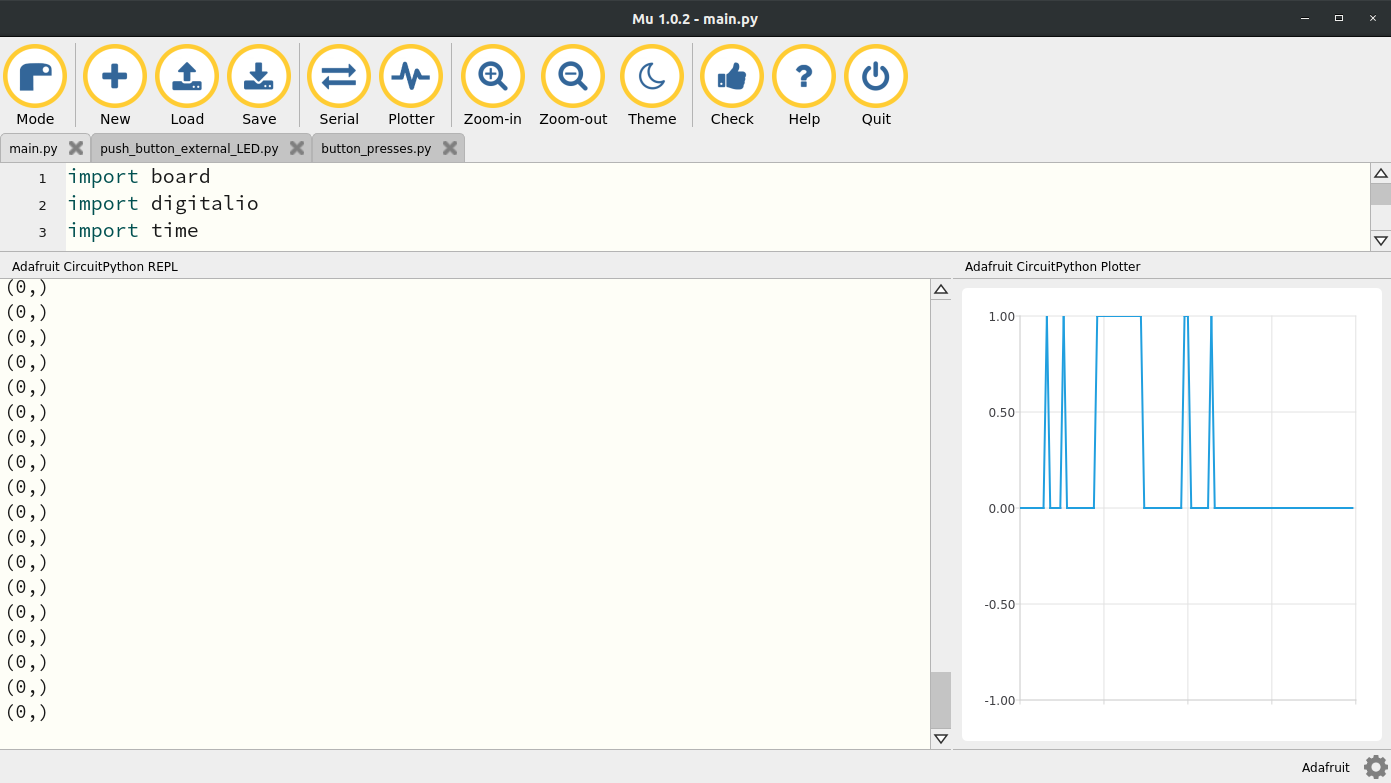
\includegraphics[width=\textwidth]{Figures/MuPlotter.png}
  \end{center}
\end{figure}
The problem with this is we still can’t save the recorded data
anywhere. Before we get into saving data let’s first edit the print
statement again to get rid of the Plotter by removing the extra
parentheses and add time.monotonic() that way we can keep track of
when a button was pressed. My print statement looks like this now: 
\begin{verbatim}
print(time.monotonic(),int(buttonA.value))
\end{verbatim}
Looking at the serial monitor now you’ll see that time is being
printed alongside the button presses. 
\begin{figure}[H]
  \begin{center}
    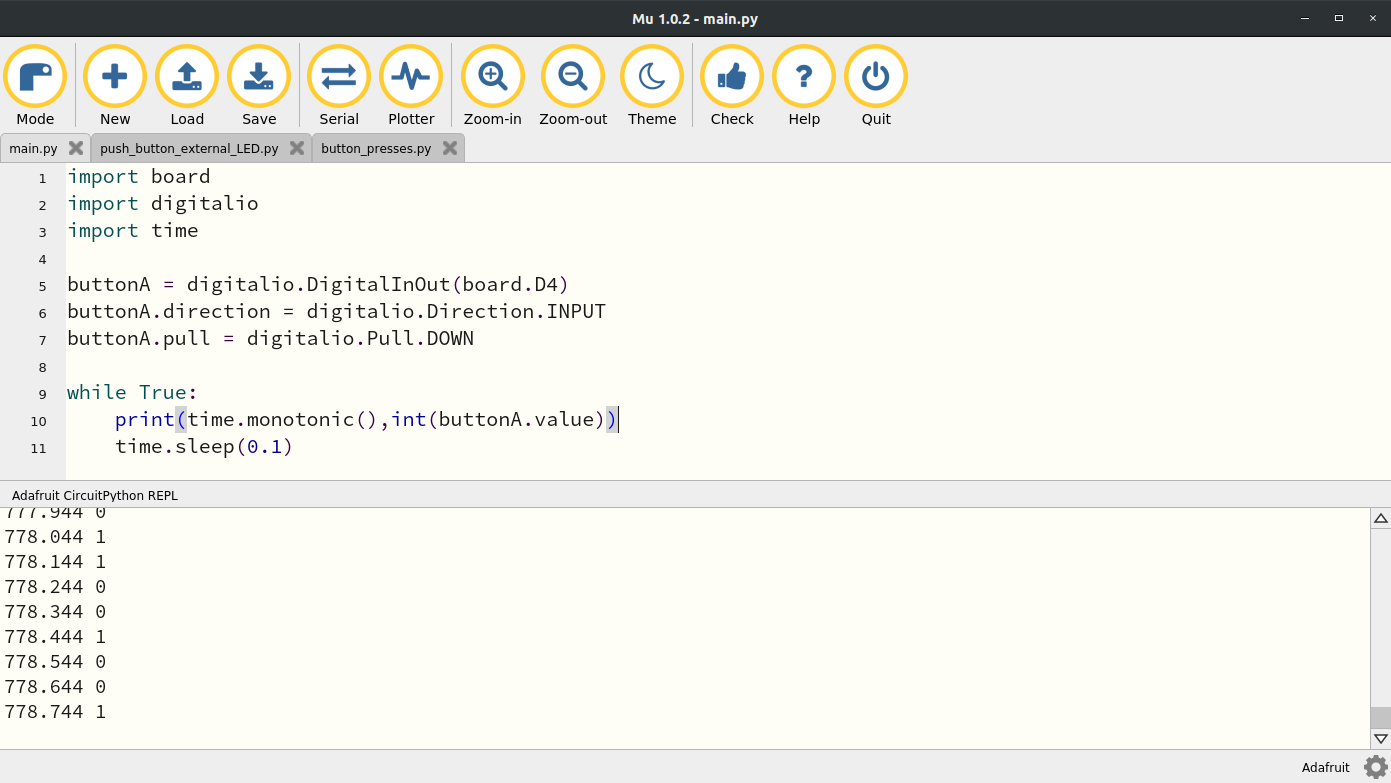
\includegraphics[width=\textwidth]{Figures/MuPlotterTime.png}
  \end{center}
\end{figure}
Now we are in a position where we can record some data and save it to
our computer. There are 4 ways to record data. I call the first,
Method1 and you basically just copy and paste from the serial monitor,
Method2 where you have the CPX/CPB type data into a spreadsheet and
Method3 where you log data internally onto the CPX/CPB itself. The 4th
method called Method4 utilizes the Bluetooth Module. Since that has
it's own issues there is a completely separate section on how to
explain Bluetooth (See section \ref{s:Bluetooth}). Note you can only
do Bluetooth if you have the Circuit Playground Bluefruit (CPB). 

\subsection{Method 1 - Copying Serial Monitor Data}

If you open up the serial monitor you can see the data output. If you
unplug the CPX while it’s taking data the code will stop. {\bf Note: In
newer versions, unplugging your CPX will result in a loss of data. If
this happens try pressing CTRL+C after you click the REPL window.} With
the code stopped you can select all the data in the Serial monitor and
then copy and paste the data into a text file on your computer. You
can actually copy this into a new file on Thonny and just save it as a
*.txt file. Once you have the data in a text file you can proceed to
plotting in Python on your desktop which I discuss in the last
section.Here’s some example data in Gedit which is a simple text
editing program.
\begin{figure}[H]
  \begin{center}
    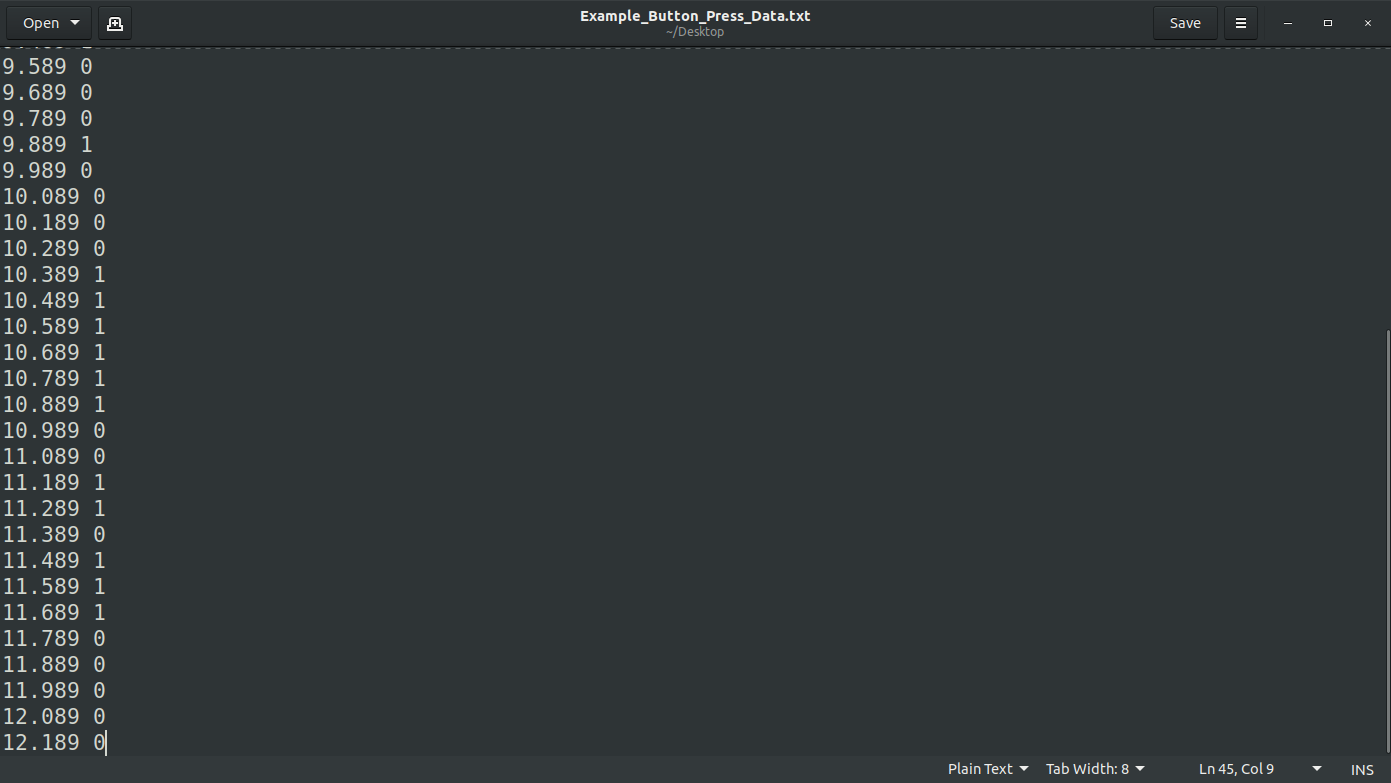
\includegraphics[width=\textwidth]{Figures/Gedit_Data.png}
  \end{center}
\end{figure}

\subsection{Method 2 - Automatically Populate a Spreadsheet}

The downside with the above method of course is if you have a ton of
data to record you could lose the data or run into a massive copy and
paste issue. The second option is to use this module called keyboard
which takes control of your keyboard on your desktop computer and
actively types your data into a spreadsheet. The code is very
extensive but I’ll include the simple one here so we can discuss
it. Below are the first 30 lines of code. The first 6 lines of code
are just comments since I heavily adopted this code from the \href{https://learn.adafruit.com/make-it-a-keyboard/circuitpython}{Adafruit
Learn System}. \href{https://github.com/cmontalvo251/Microcontrollers/blob/master/Circuit_Playground/CircuitPython/Data_Logging/typing/record_button_presses_typing.py}{My version of this code} can be found on my Github. Lines 8 -
14 are import commands as we’ve seen previously. The regular import
modules board, time and digitalio are imported but we are also
importing the Keyboard module so that the CPX can takeover our
keyboard. Lines 16-22 create two buttons. First we create buttonA
attached to pin D4 and then a switch attached to pin D7. If you look
on the CPX there is a switch labeled D7. Before you copy this code
onto the CPX make sure you move the switch towards the ear looking
symbol. Lines 26-28 created the keyboard object. We are going to call
it layout for this example code.
\begin{figure}[H]
  \begin{center}
    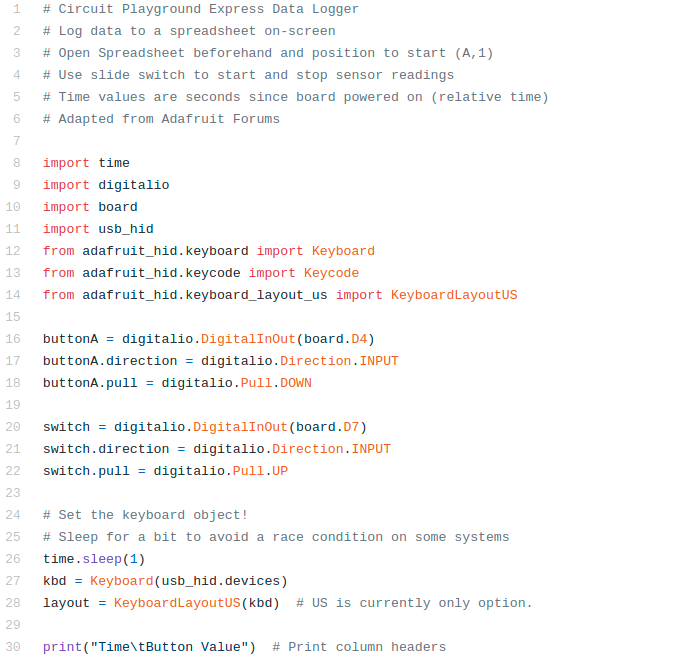
\includegraphics[width=\textwidth]{Figures/Typing1.png}
  \end{center}
\end{figure}
The next 30 lines are shown below. Lines 32-35 define a
function. Functions in Python have a pretty standard structure. The
keyword def is used to denote that the next line is a definition for a
function. The name of the function is {\it slow\_write()}. The input to the
function is string which ironically enough is a string object. Line
33-35 define what the function does. Line 33 sets up a for loop where
the code loops through each character in the string. Everytime it gets
to a new character it will use your keyboard to type that character
using the layout.write(c) command. The time.sleep(0.02) is just to
slow down the keyboard so your computer can keep up. That function is
defined above the standard while True: statement on line 37 but is
called on line 42. You’ll see there is a {\it slow\_write(output)} on line
42. In this case output is a string and it’s sent to the function
{\it slow\_write()}. So in this case we have a function that can write a
string so we just need to take data and then write it using our
keyboard. Line 38 is an if statement that will only be true if the
switch on pin D7 is pushed towards the music note on the CPX. If the
switch is not thrown the code will move to the else statement on line
52 and tell the user that you need to flip the switch. If the switch
is thrown line 40 will take data for us. First it will record the
time.monotonic() and store it as a floating point number using the
\%0.1f designation which means that it will store 1 decimal as a
\%floating point number for f.
\begin{figure}[H]
  \begin{center}
    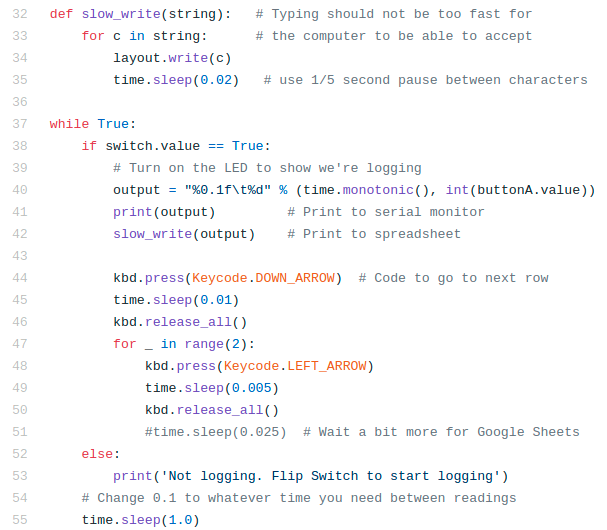
\includegraphics[width=\textwidth]{Figures/Typing2.png}
  \end{center}
\end{figure}
The second number in the string is an integer or a base 10 (decimal)
integer designated by the \%d part of the format. The integer is
int(buttonA.value). You’ll see a \t in between the formatted numbers
which is a tab. The tab is there to tab between cells in a
spreadsheet. Line 41 will print the output string to the Serial
monitor and it will also type the contents of the string. Very
important here. When you flip the switch on the CPX your keyboard will
start typing in whatever active window is selected. If you don’t have
a spreadsheet opened and active (selected), the keyboard will just
begin typing in whatever window is open. Make sure you have a
spreadsheet program open and ready to go. Lines 44-51 tell the
keyboard to hit the {\it DOWN\_ARROW} on your keyboard to move to the next
row and the {\it LEFT\_ARROW} twice to move back to the first column. Line 55
is a sleep to only log data once a second. I ran this code for a bit
and had it type into LibreOffice Calc which is a free spreadsheet
program. Google Sheets or Microsoft Excel will also work just fine. 
\begin{figure}[H]
  \begin{center}
    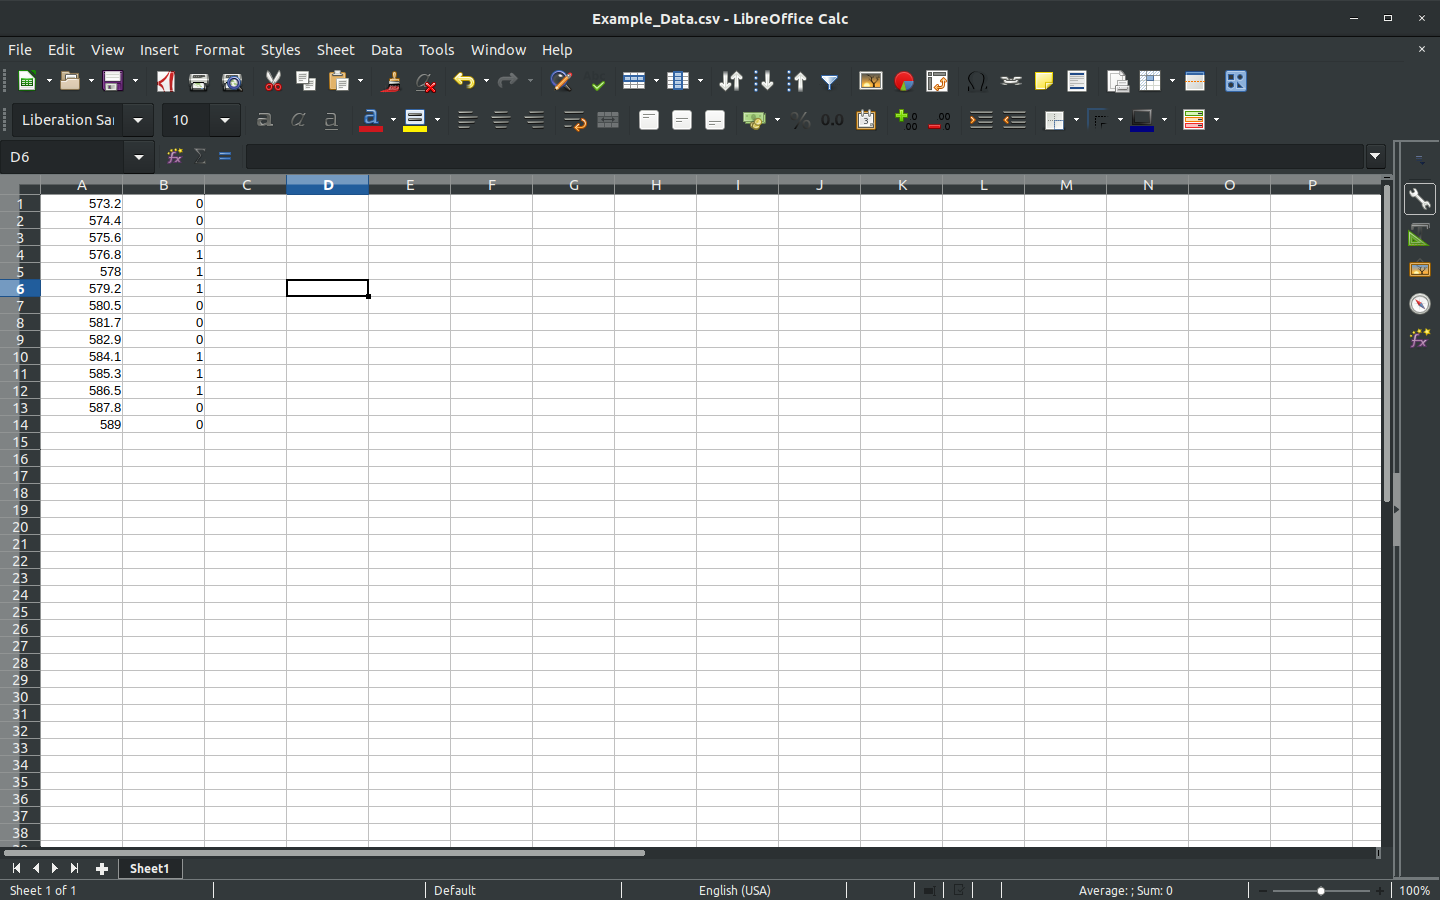
\includegraphics[width=\textwidth]{Figures/Typing3.png}
  \end{center}
\end{figure}
You’ll see that the first column is time with 1 decimal point and the
second column is the button press values. At this point you must click
{\it Save As...} and save the document as a CSV which stands for Comma
Separated Value. Once you have the file saved you can proceed to
plotting in Python on your Desktop. 

\subsection{Method 3 - Logging Data Directly to on board memory}

The problem with the above 2 methods is that you need a laptop to log
data in the field. It would be nice if you could use the optional
battery pack and just have the CPX log data on the CPX itself. This is
the most complex way but in my opinion the best way. In order to get
this to work you need to allow the drive on the CPX to have read/write
permissions. This requires you to load a piece of software called
boot.py and put it on the CPX. I have this
\href{https://github.com/cmontalvo251/Microcontrollers/blob/master/Circuit_Playground/CircuitPython/Data_Logging/boot.py}{software
  on my Github}. The software is shown below. The first 10 lines are
probably very familiar. Import some modules and then create a switch object. Line 13
is where all of the storage permissions are changed. If the flip is
switched towards the A button, the storage module is used to allow you
to write to the CPX. The problem here is that if you do this, you
won’t be able to edit code. I’ll explain the procedure here in a
minute. As always, the relevant Adafruit tutorial is on the \href{https://learn.adafruit.com/adafruit-circuit-playground-express/circuitpython-storage}{Adafruit
Learn System} if you want to read more about it. Again make sure you
store this file onto the CIRCUITPY drive and save it as boot.py
\begin{figure}[H]
  \begin{center}
    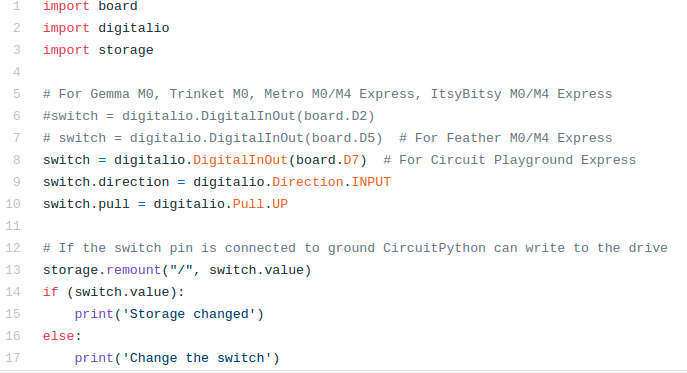
\includegraphics[width=\textwidth]{Figures/boot.png}
  \end{center}
\end{figure}
In addition to storing the file boot.py you’ll need to edit your
main.py script to only log data when the switch is moved towards the B
button. The software to record button presses on disk is shown below
and as always
\href{https://github.com/cmontalvo251/Microcontrollers/blob/master/Circuit_Playground/CircuitPython/Data_Logging/write_button_presses_disk.py}{on
  my Github}. In this software we again see the standard 
commands. Lines 1-3 import all the modules we need and then 5-15
create a switch, a button and an LED. In this case we’re using the LED
soldered to the board. Line 17-20 check to see if the user has flipped
the switch. If the switch is False the storage module on boot.py will
allow the drive to act like a data logger and it will open a file
called {\it Test\_Data.txt} for writing (‘w’). If the switch is True then the
user will be notified that the file has not been opened for
writing. Lines 22 through 33 include the infinite while loop. Line 23
turns the LED on and line 24 prints out the current time and the
button value in integer form. If the switch value is False the program
will create an output string by converting all numbers to strings
using the str function. Notice that there is a {\it
  str(``\textbackslash n")} at the end of
the output variable which tells the computer to write a new line of
data to the file. Lines 28 and 29 write the output to the file from
line 18 and then flush the output which means the CPX waits for the
data to be fully written before moving on. It also turns the LED off
so we know the CPX took data even when we aren’t looking at the Serial
monitor. If the switch value is true it means that the we never opened
the data file and thus we tell the user we aren’t logging data and
it’s time to flip the switch and hit reset. {\bf NOTE: The figure below is from an old version of the code. The newest version produces the same outcome. The only difference is that the D13 LED blinks when the code is running and the first neopixel toggles 3 different colors when the system is logging data. This allows for extra user information when operating Method 3 without a computer and the serial monitor. Note that these additions require the use of neopixel.mpy module.} {\bf One issue you're going to run into when
you run the codes below is that you won't have some of the modules on
your CPB/CPX.} To fix this you need to download
the \href{https://circuitpython.org/downloads}{CircuitPython
Modules}. You need to click the CircuitPlayground Express or Bluefruit
depending on which one you have and then download the appropriate
version: 6.x, 7.x or 8.x. How do you know what version of CircuitPython
you have? Well head over to your CIRCUITPY drive and open the
boot\_out.txt file and it will tell you the version. Note that this is
the same version as the .UF2 file installed back in the Getting
Started labs (See Chapter \ref{s:Getting_Started}). When you download
the modules it will download a .zip file. Extract the .zip file on
your desktop computer and then open the {\it lib} folder on your
desktop and your CIRCUITPY. You then need to transfer the modules
(ONLY THE ONES YOU NEED) from your desktop to your CPX/CPB. The reason
why you can't copy the entire folder is because the CPB/CPX only has
2MB of flash and the CircuitPython download is 4.1 MB at the time of
this writing. 

\begin{figure}[H]
  \begin{center}
    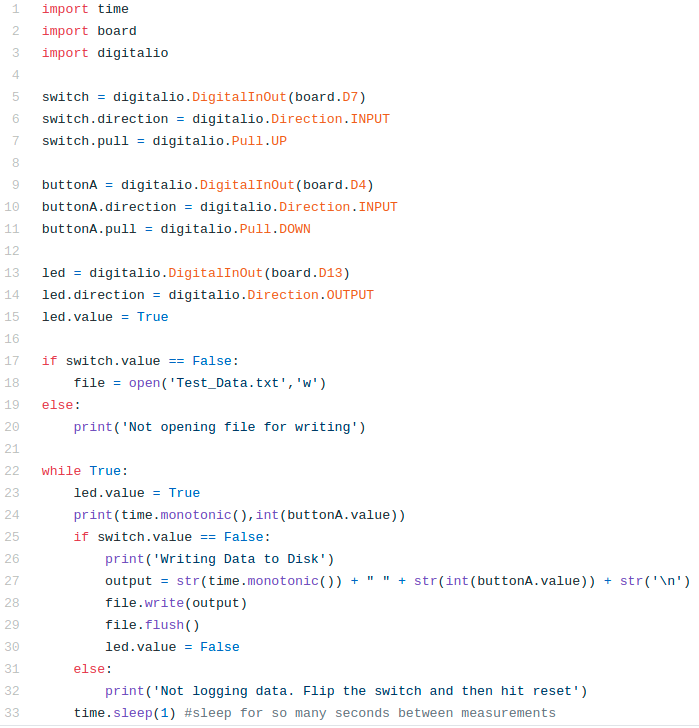
\includegraphics[width=\textwidth]{Figures/method3_1.png}
  \end{center}
\end{figure}
So here is the flow of what you want to do for method 3.
\begin{enumerate}[itemsep=-5pt]
\item Unplug the CPX
\item Flip the switch towards the A button.
\item Plug in the CPX and save the boot.py and main.py files. Remember you can only save Python scripts when the switch is flipped towards the A button.
\item When you are ready to start recording data, flip the switch towards the B button. If you’re looking at the Serial monitor, the software will throw an error. Just ignore it and hit the reset button. When your computer recognizes the CPX you can turn the Serial monitor on and off.
\item When you are done taking data simply slide the switch over towards the A button and hit reset again. This is what my Serial monitor looks like when I do this. You’ll see that I was writing to disk for like 25 seconds and then I flipped the switch back towards the A button.
\end{enumerate}
\begin{figure}[H]
  \begin{center}
    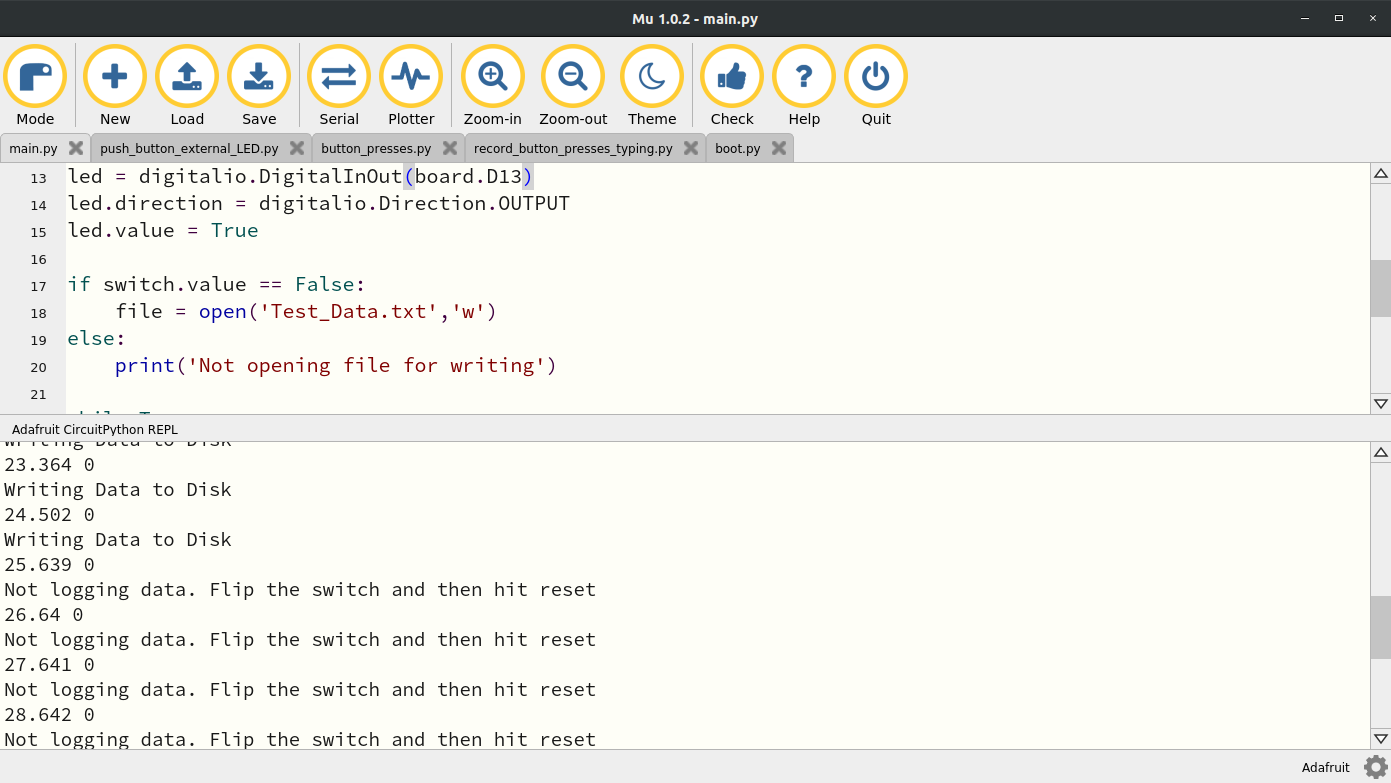
\includegraphics[width=\textwidth]{Figures/method3_2.png}
  \end{center}
\end{figure}
With the switch flipped and data taken, open your folder manager and
take a look at the CIRCUITPY drive. This is what mine looks
like. You’ll see I have two Python files and a file {\it Test\_Data.txt} with
all my data in it. 
\begin{figure}[H]
  \begin{center}
    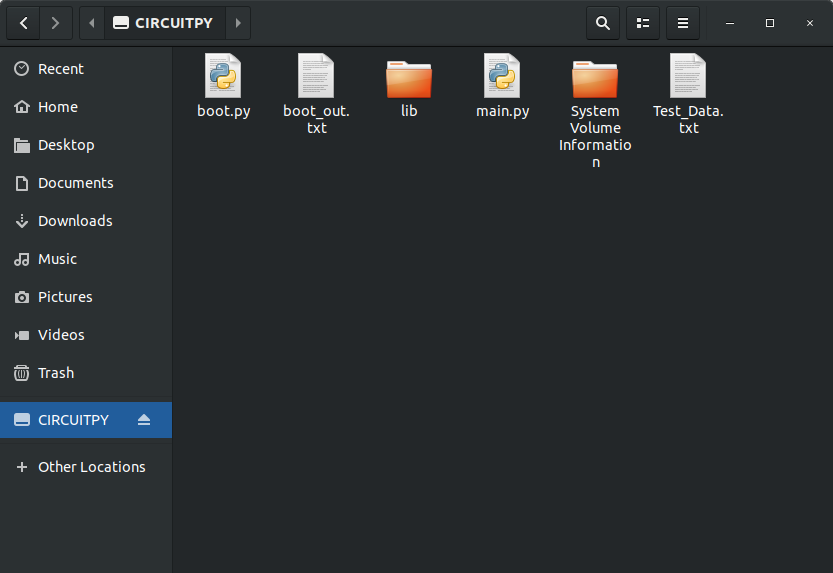
\includegraphics[width=\textwidth]{Figures/method3_3.png}
  \end{center}
\end{figure}
If you open the {\it Test\_Data.txt} file you will hopefully see data in it.
\begin{figure}[H]
  \begin{center}
    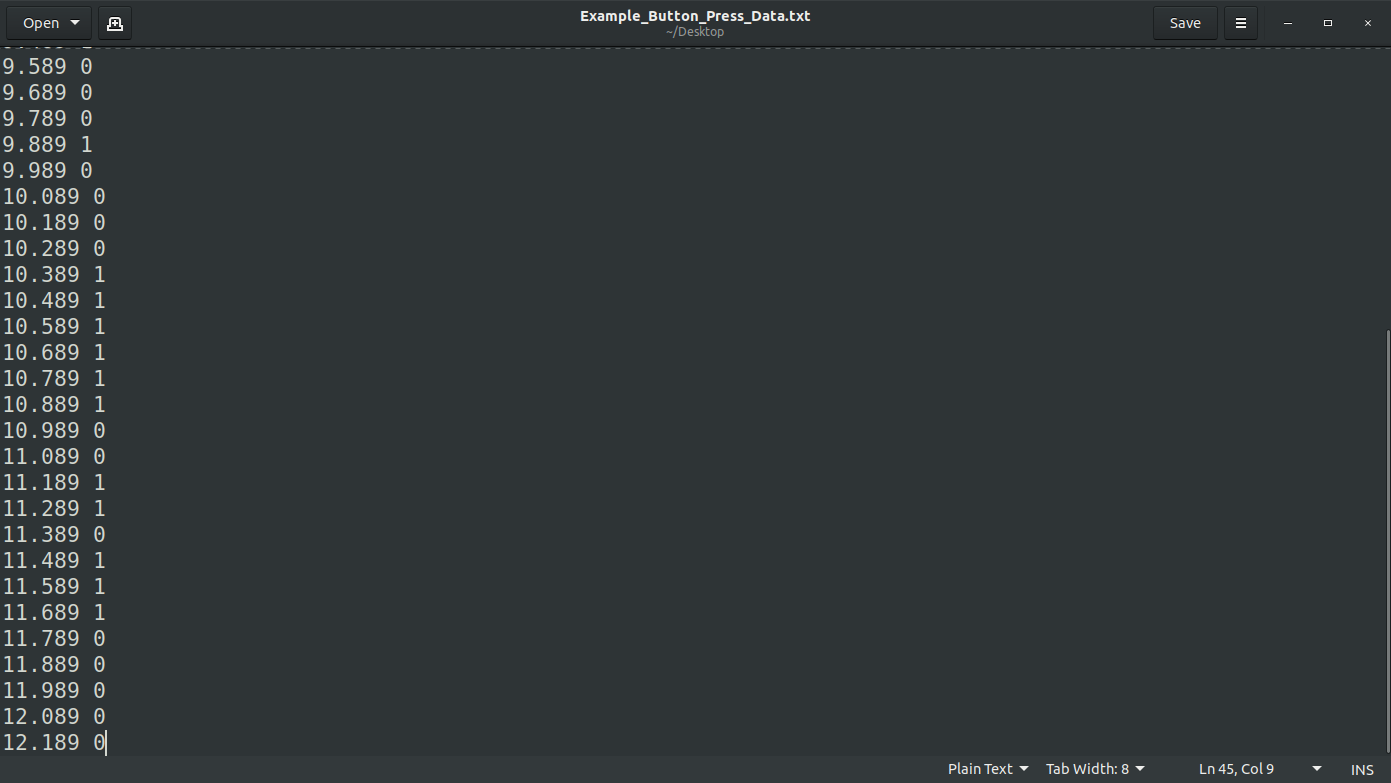
\includegraphics[width=\textwidth]{Figures/Gedit_Data.png}
  \end{center}
\end{figure}
At this point you can copy this text file over to your desktop computer and proceed to the Python plotting portion.
Ok so let’s recap method 3 one more time.
\begin{enumerate}[itemsep=-5pt]
\item Unplug CPX (or remove power)
\item Slide switch to A
\item Plug in CPX (or provide battery power)
\item Slide switch to B
\item Reset
\item Take data for however long you want
\item Slide switch to A
\item Remove power if you’re on battery power
\item Plug CPX into computer if not already connected
\item Transfer data file to computer
\end{enumerate}

\subsection{Method 4 - Logging Data on a Cell Phone using Bluetooth
(CPB Only)}

As mentioned in the introduction it's possible to have the Circuit
Playground send data wirelessly to a cell phone using Bluetooth
provided you have Bluetooth setup and a smart phone with the Adafruit
Connect App. Bluetooth is explained in detail in its own section (See
Section \ref{s:Bluetooth}). Method 4 is a valid form of logging data
it just requires a cell phone to be powered the entire time and it
must be within 30 feet of the Circuit Playground at all times. This
also only works on the CPB since the CPX does not have a Bluetooth
transmitter. 

\subsection{Plotting Logged Data}

Alright so there you have it. I have explained 4 methods to
datalogging. Here are the methods again in summary.

\begin{enumerate}[itemsep=-5pt]
\item Print data to Serial and copy and paste
\item Use the Keyboard module to save data to a spreadsheet
\item Access the storage of your CPX and write data to a text file on
the CPX
\item Send data wirelessly to a Cell Phone using Bluetooth - CPB Only (See
Section \ref{s:Bluetooth})
\end{enumerate}

All methods will work but some will obviously have their pros and
cons. I suggest you get comfortable with 1 method and use that for the
remainder of the semester. Whatever option you choose though will
provide you with a data file that you can read in Python on your
desktop computer to plot. The simplest way to import data is by using
the loadtxt function from the module numpy. Here is some very simple
code to plot data from a text file. I also have a \href{https://www.youtube.com/watch?v=tJOz-ty-2ec&list=PL_D7_GvGz-v1RsDs_OdNW65qRjEjmpfQx&index=12}{Youtube video
explaining how to plot a text file} if you’d rather watch something. 

When you plot make sure your {\it Test\_Data.txt} file is in the same folder
as your plotting script in Thonny or Spyder. Here’s my example code
(this code is not on Github but you only need 3 or 4 lines of code to plot). 
\begin{figure}[H]
  \begin{center}
    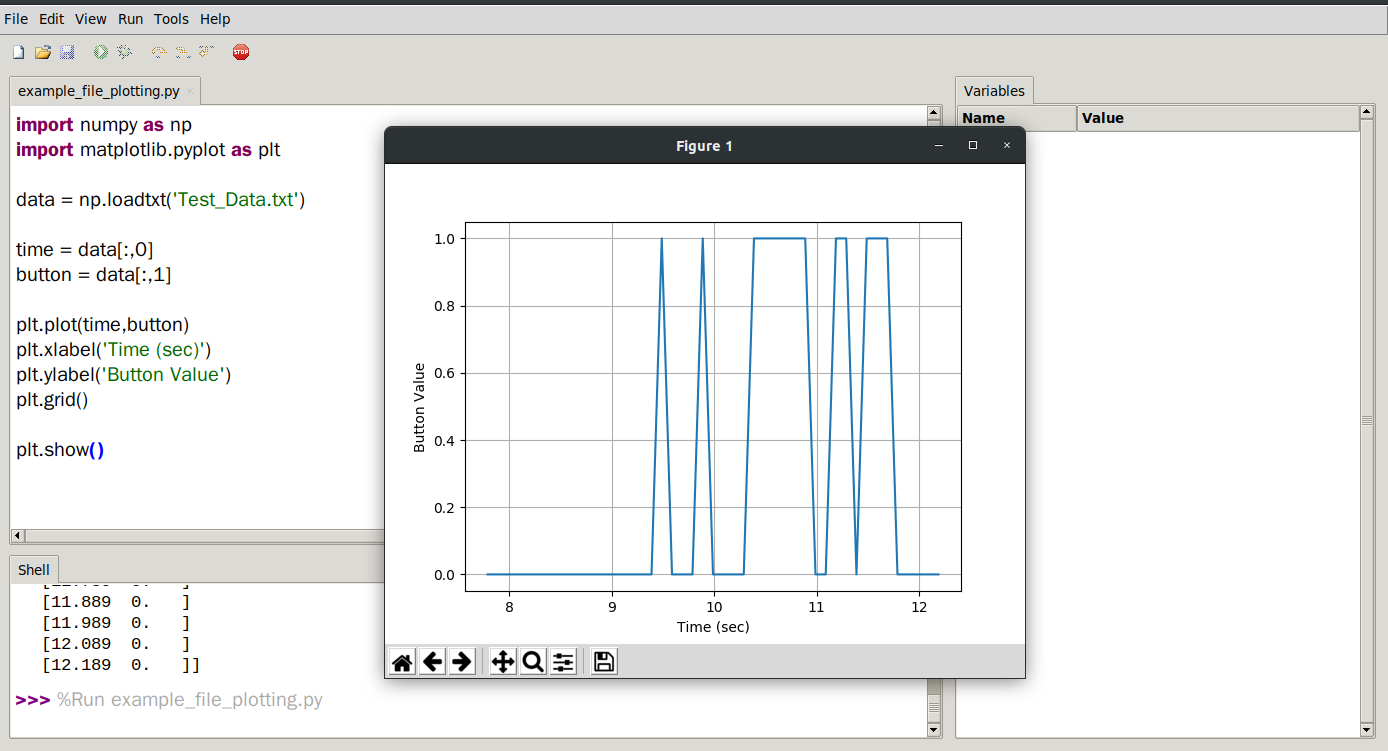
\includegraphics[width=\textwidth]{Figures/plotdata.png}
  \end{center}
\end{figure}
In this example lines 1 and 2 import numpy and matplotlib. Line 4
imports data from the {\it Test\_Data.txt} file and then 6 and 7 save the
first and second columns into time and button. The remaining lines
plot the data and create x and y labels as well as a grid. Hopefully
now you are well versed in taking data and plotting in Python.

\subsection{Assignment}

Once you've completed the project above, upload a PDF with all of the photos and text
below included. My recommendation is for you to create a Word document
and insert all the photos and text into the document. Then export the
Word document to a PDF. For videos I suggest uploading the videos to
Google Drive, turn on link sharing and include a link in your
PDF. Note that all code must be included in the appendix or you'll be
penalized 10\%. 


\begin{enumerate}[itemsep=-5pt]
\item Use method 1, 2 or 3 and save time and button presses to a text file
\item Include a video explaining which method you are using to record button presses and show yourself pressing the CPX button a few times and recording data. Make sure to wave and introduce yourself - 30\%
\item Copy and Paste your CPX code used to log data - 20\%
\item Copy and paste your Python desktop code used to plot your data - 20\%
\item Include a plot of your button presses with time on the x-axis and button presses on the y-axis (no screenshots) - 30\%
\end{enumerate}
